\chapter{Plant functional types mapping}
We proposed a combined machine learning approach with a deep convolutional neural network (CNN) to monitor forest utilization toward Sustainable Development Goals (SDGs) for data-scarce regions. First, we employed the Random Forest (RF) classifier using Google Earth Engine (GEE) for forest mapping. Then, we designed a deep CNN architecture that works for PFTs/age mapping from coarse and polygonal ground-truth data. The proposed network has U-shape and comprises 3D Atrous Convolutions. The model was optimized by a weighted cross-entropy loss function. We trained the model with times-series Sentinel 1, 2, and Digital Elevation Model (DEM) data with sparse annotations. Our proposed models achieved 94.5\% overall accuracy (OA) for forest mapping, 77.80\% (OA) for PFTs, and 81.74\% (OA) for forest age classification, respectively in Ena city, Japan. The outcome of our study indicates the potential of remote sensing and machine learning in monitoring forest development, conservation, and utilization toward SDGs from coarse ground-truth data. Our source code for the implementation is available at: \url{https://github.com/anhp95/forest_attr_segment}
\renewcommand{\headrulewidth}{0pt}
\lhead[\thepage]{\leftmark}
\rhead[\leftmark]{\thepage}
\cfoot[]{}

\section{Introduction}
The pivotal role of forests in advancing Sustainable Development Goal 15 (SDG15) and addressing global climate change is widely recognized. Leveraging the capabilities of remote sensing technology and cutting-edge machine learning algorithms, the mapping of forested areas, along with the identification of PFTs and forest age, emerges as a valuable contribution to the monitoring of SDG-related issues, encompassing indicators such as 15.1.1, 15.2.1, and 15.4.2. \par

While forest mapping is a familiar task in land-cover/land-use classification, generating a detailed map specifying plant functional types (PFTs) and forest age introduces heightened complexity. Previous studies focusing on PFTs/age classification often relied on either high-resolution input data or ground-truth information at the point level, as evidenced in the works of \citep{schiefer2020mapping,la2021multi, lee2016individual}. However, these resources are known to be expensive, time-consuming to collect, and infrequently available in specific regions, particularly in developing areas. In response to these challenges, this chapter introduces a methodology aimed at monitoring forest areas, PFTs, and forest age, utilizing coarse annotations and freely available remote sensing data. \par

The approach begins with the application of a Random Forest (RF) classifier to classify forested areas. Subsequently, a deep Convolutional Neural Network (CNN) architecture is designed for the segmentation of PFTs and forest age. Notably, our proposed methodology demonstrates its efficacy in regions where data scarcity is a significant concern. \par

The structure of this chapter unfolds as follows: Section \ref{chap5_data} provides insights into the study area and the data utilized in the study. Section \ref{chap5_method} delves into the overall methodology employed, and the experimental results within the study area are expounded upon in Section \ref{chap5_result}. Finally, Section \ref{chap5_conclusion} encapsulates the conclusion of the chapter, highlighting avenues for future research and development. \par

\section{Data} \label{chap5_data}
\subsection{Study area}
The focal point of our investigation is Ena city (see Figure \ref{fig:chap5_studyarea}), strategically positioned in the southeastern expanse of Gifu prefecture, nestled within the heart of Japan. Encompassing an expansive total area of approximately 504 square kilometers, the city boasts an elevation of 282 meters, contributing to its diverse topography. The climate exhibits a noteworthy annual temperature range, spanning from a minimum of 2 °C to a maximum of around 26.4 °C, showcasing the dynamic climatic conditions that characterize the region. \par

\begin{figure}[tbh!]
    \centering
    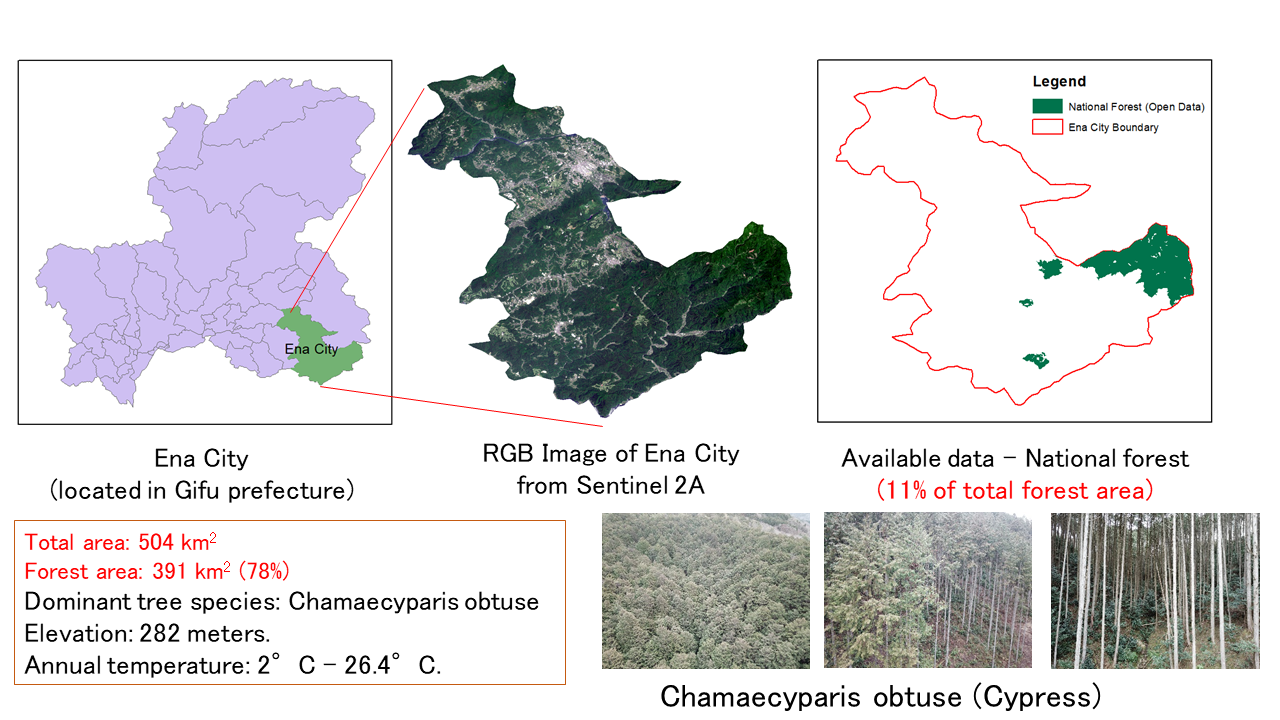
\includegraphics[width=\textwidth]{figs/chap5/study_area_ena.png}
    \caption[National forest in Ena city]{Ena city and national forest in Ena city.}
    \label{fig:chap5_studyarea}
\end{figure}

A compelling facet of Ena city lies in its rich forest cover, a significant portion of which, as reported by local government statistics, comprises artificial forests, constituting 60\% of the total forested area. The dominant species within these artificial forests is Chamaecyparis obtusa. This coniferous species plays a pivotal role in the city's ecosystem, serving multifaceted purposes such as timber production, prevention of water-related disasters, and the sequestration of carbon dioxide (CO2). Notably, the artificial forest, largely populated by Chamaecyparis obtusa, underscores its significance as a valuable resource for sustainable timber harvesting, acting as a buffer against potential water-related calamities, and contributing to the mitigation of greenhouse gas emissions through effective CO2 sequestration. This intricate interplay of environmental elements highlights the intricate web of ecological services provided by Ena city's forests, emphasizing their integral role in the broader context of regional sustainability and resilience. \par

\subsection{Data collection}
In our forest mapping approach, the creation of a training set involved a random selection of 750 forest and 250 non-forest points, alongside a validation set comprising 300 forest and 100 non-forest points. This selection was based on the 2016 land-use map provided by the National Land Information Portal. Transitioning to the task of mapping PFTs and forest age, our labeled data was sourced from the same repository. The ground-truth information, represented as coarse polygons, delineates mixed-species zones, with each polygon annotated according to the most dominant PFTs in that particular area. Notably, this ground-truth data is restricted to national forest areas, presenting a limitation in its coverage. To address this constraint, given the relatively small portion (11\%) of national forest data available for Ena city, we supplemented our dataset with the annotations collected in 2018 from Gifu prefecture to enhance model training (\ref{fig:chap5_gifu_gt}). \par


\begin{figure}[p]
    \centering
    \begin{subfigure}{\textwidth}
        \centering
        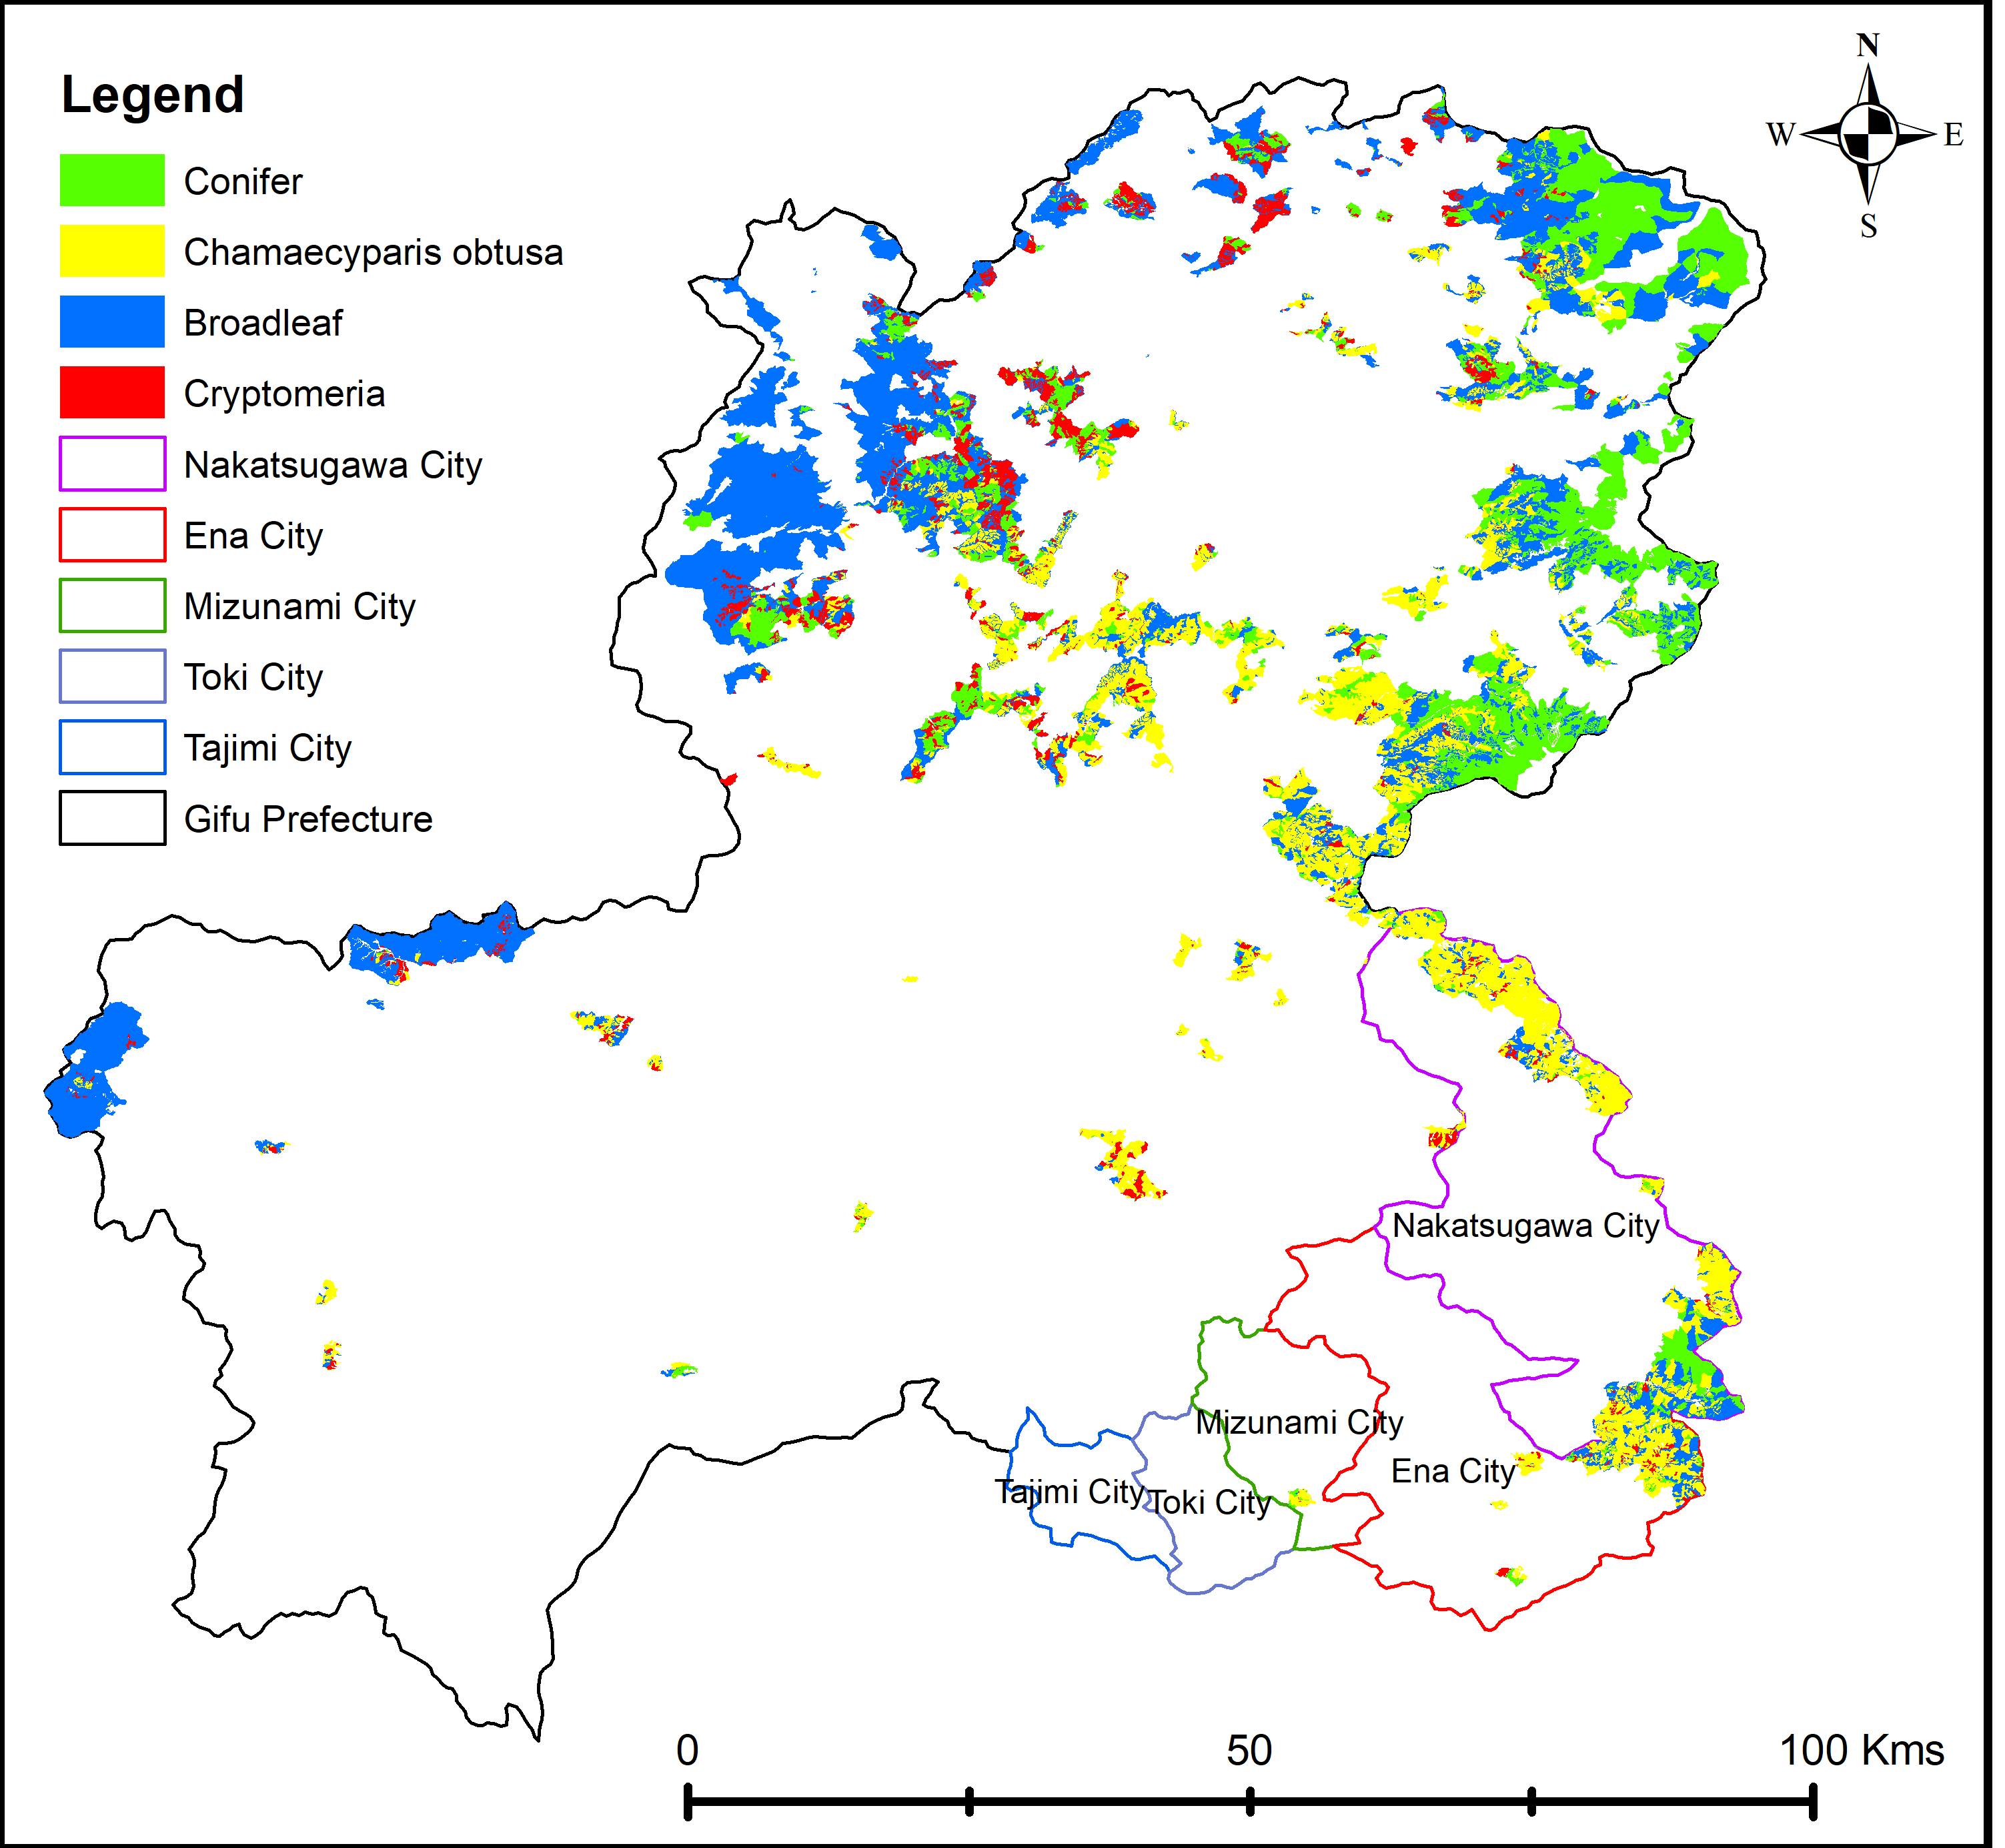
\includegraphics[width=\textwidth]{figs/chap5/gifu.png}
        \caption{Annotations of national forest in Gifu prefecture (black boundary)}
        \label{fig:chap5_gifu}
    \end{subfigure}

    \begin{subfigure}[c]{.5\textwidth}
      \centering
      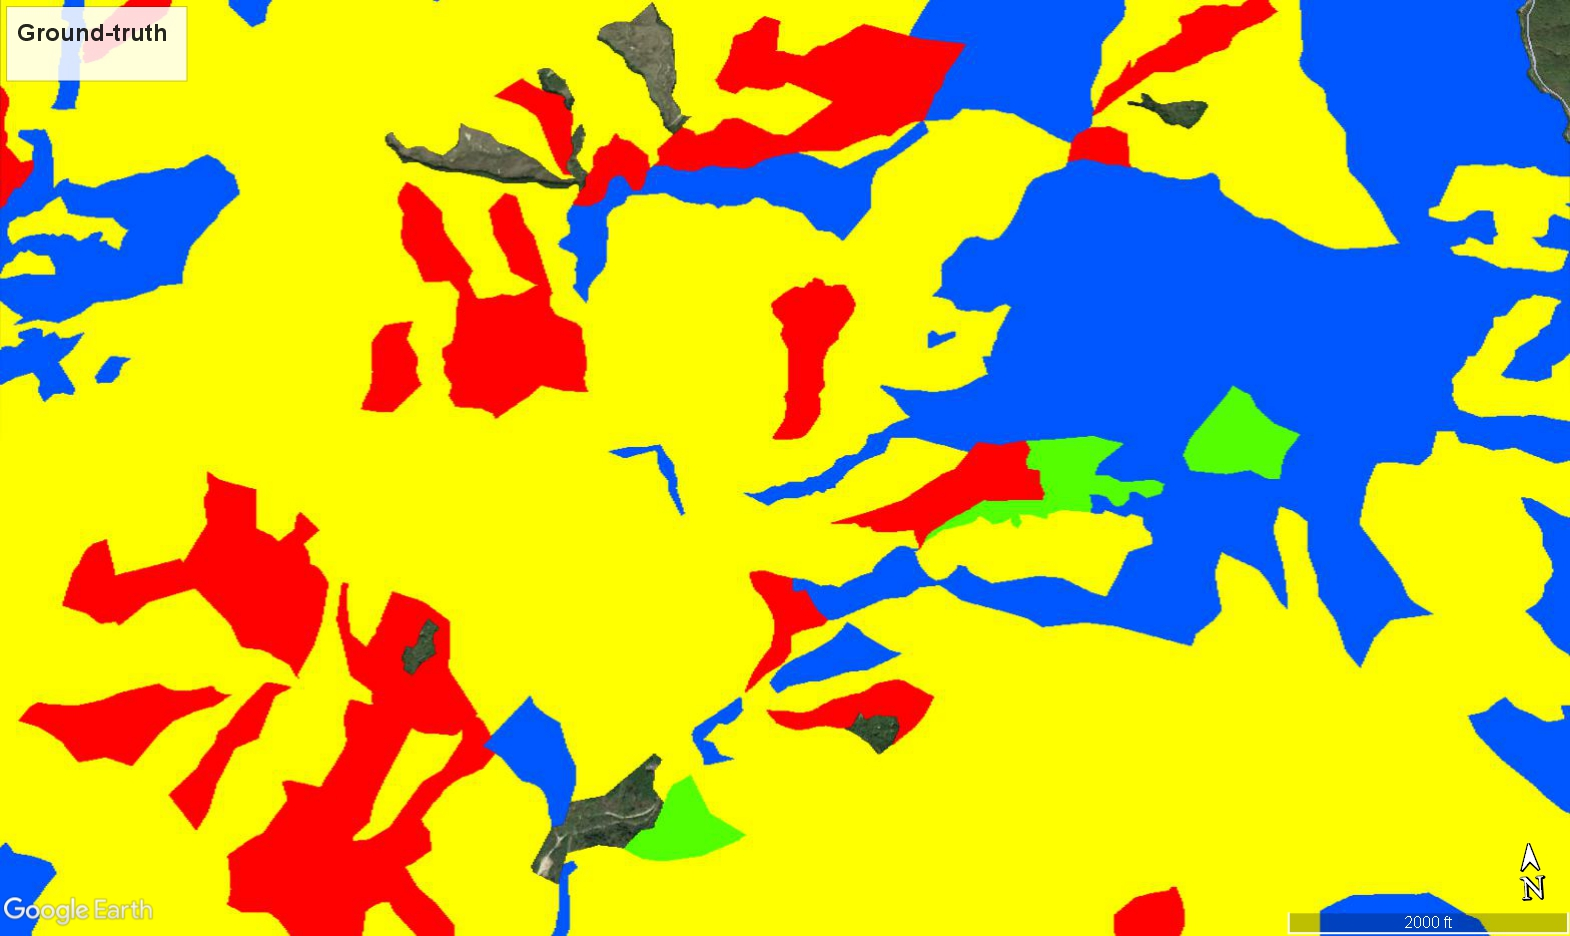
\includegraphics[width=\textwidth]{figs/chap5/gt-ge.jpg}
      \caption{Example of annotated area}
      \label{fig:chap5_gtge}
    \end{subfigure}%
    \begin{subfigure}[c]{.5\textwidth}
      \centering
      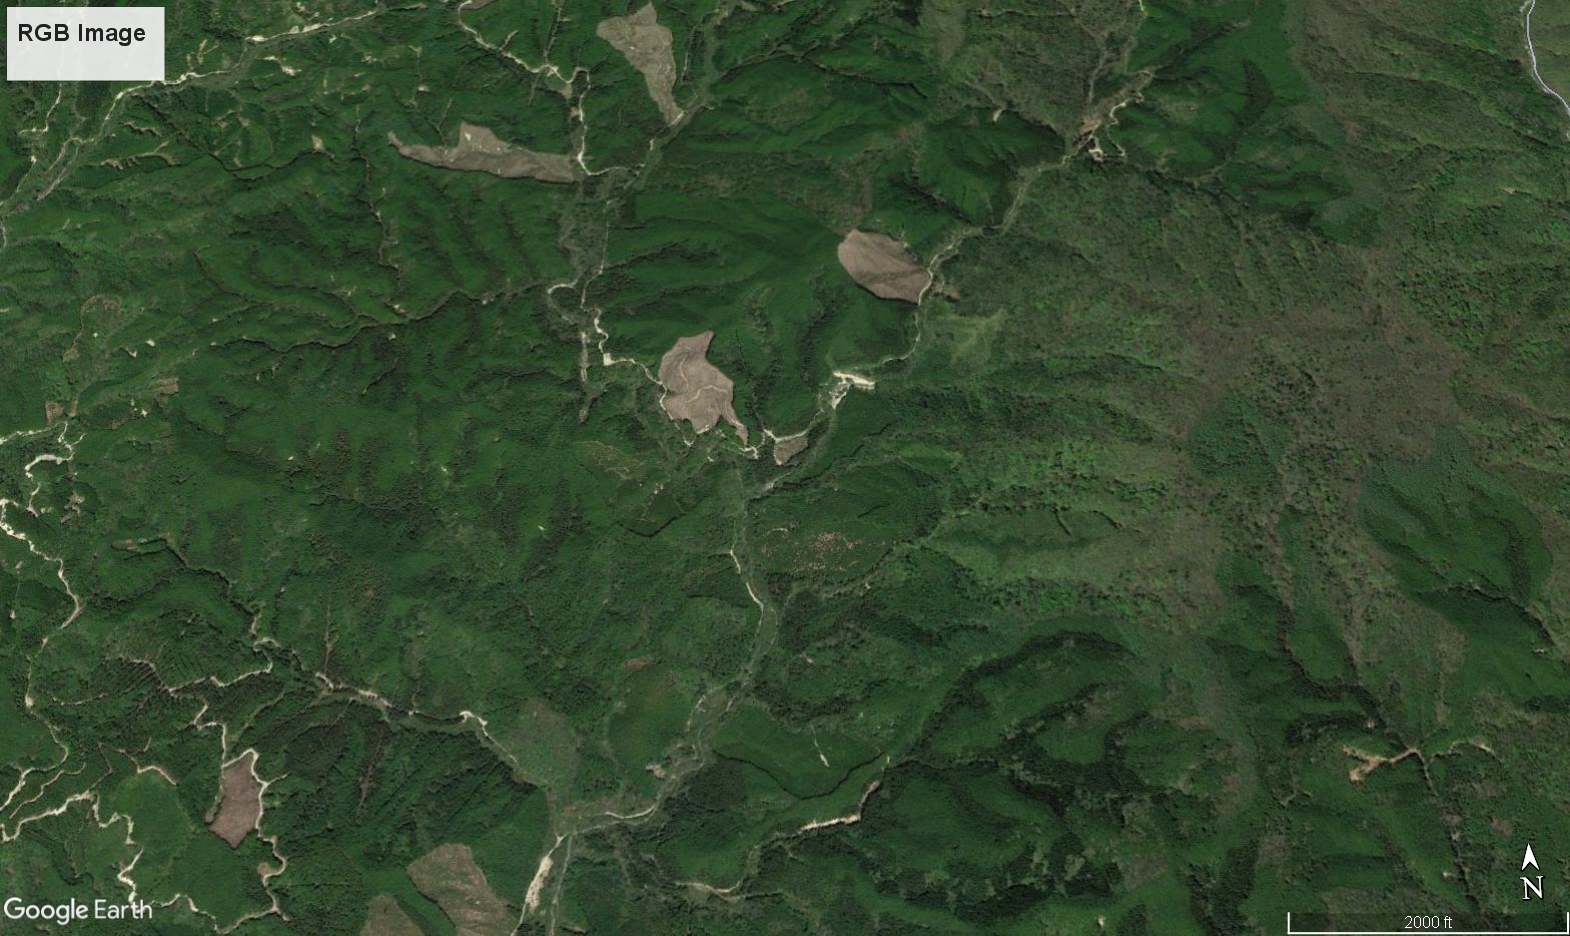
\includegraphics[width=\textwidth]{figs/chap5/gt-rgb.jpg}
      \caption{The corresponding RGB image}
      \label{fig:chap5_gtrgb}
    \end{subfigure}
    \caption[Study area and annotated data]{(a) The designated study area outlined in red is Ena city, (b) demonstrates coarse annotations as an illustrative example, and (c) showcases the corresponding RGB image sourced from Google Earth.}
    \label{fig:chap5_gifu_gt}
\end{figure}

Our utilization of remote sensing resources encompassed Sentinel 1A, Sentinel 2 L1C, and a Digital Elevation Model (DEM), each featuring  spatial resolutions of 10m, 10m, and 30m, respectively. The dataset comprises 11 spectral channels, encompassing the Red, Green, Blue, Red Edge, Near-infrared, Short-wave infrared, and Normalized Difference Vegetation Index (NDVI) from Sentinel 2, along with the VV and VH bands from Sentinel 1A. Additionally, the DEM data is derived from the NASA Shuttle Radar Topography Mission digital elevation model, providing crucial elevation information. This comprehensive dataset serves as the input features for our machine learning model.\par

In the subsequent sections, we describe the specifics of acquisition times for Sentinel 1 and Sentinel 2, pertaining to the segmentation of PFTs and forest age, as well as forest mapping. Recognizing the dynamic nature of forest ecosystems and evolving land-use patterns, the temporal dimension of data acquisition plays a crucial role in maintaining the relevance and accuracy of our models. \par

\section{Methodology} \label{chap5_method}
The proposed workflow is depicted in Figure \ref{fig:chap5_workflow}. Initially, the Sentinel 1 data was obtained directly from Google Earth Engine (GEE). Each pixel represents the backscatter coefficient and undergoes a series of preprocessing steps, including the application of an orbit file, removal of GRD border noise, thermal noise elimination, radiometric calibration, and terrain correction. The Sentinel 2 data was mosaicked and monthly averaged to address clouds and missing values, also leveraging GEE. The training and validation sets for forest mapping, Plant Functional Types (PFTs), and forest age segmentation were extracted from the satellite images. Subsequent sections provide a detailed illustration of how these acquired sets are utilized to train the machine learning models. \par


\begin{figure}[p]
    \centering
    \begin{subfigure}{\textwidth}
        \centering
        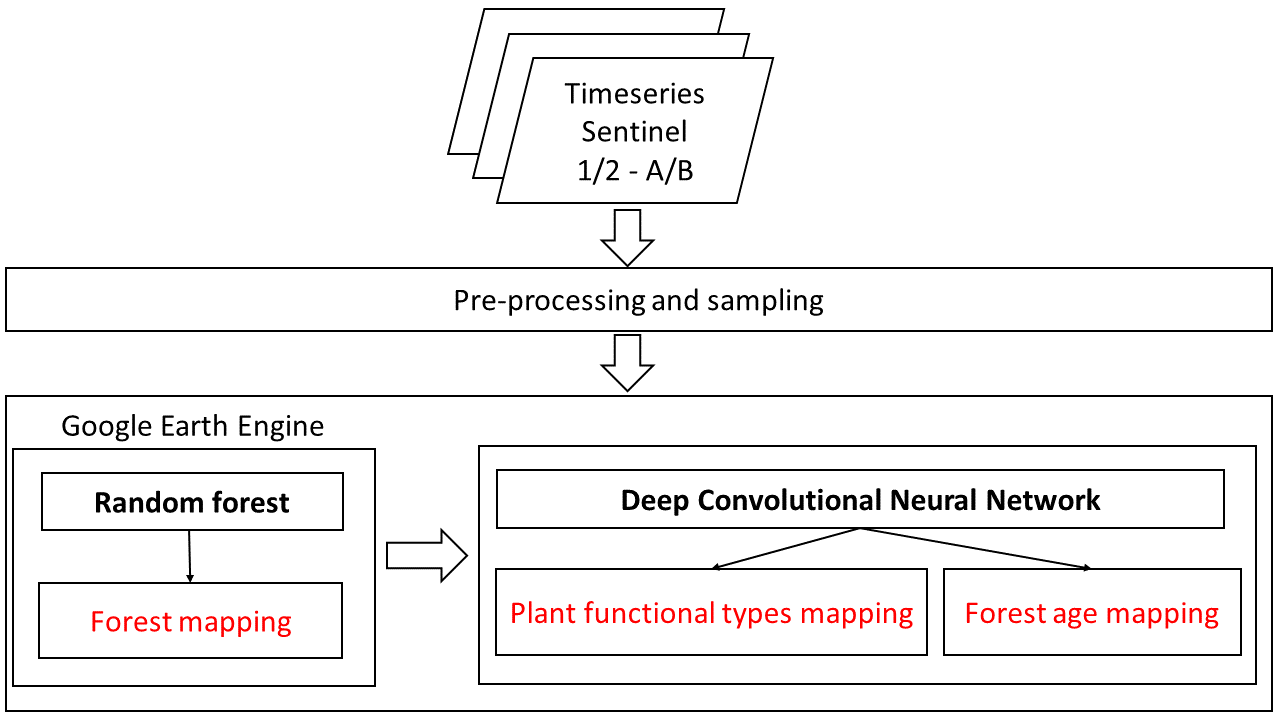
\includegraphics[width=\textwidth]{figs/chap5/workflow.png}
        \caption{Overall Workflow}
        \label{fig:chap5_workflow}
    \end{subfigure}

    \begin{subfigure}{\textwidth}
        \centering
        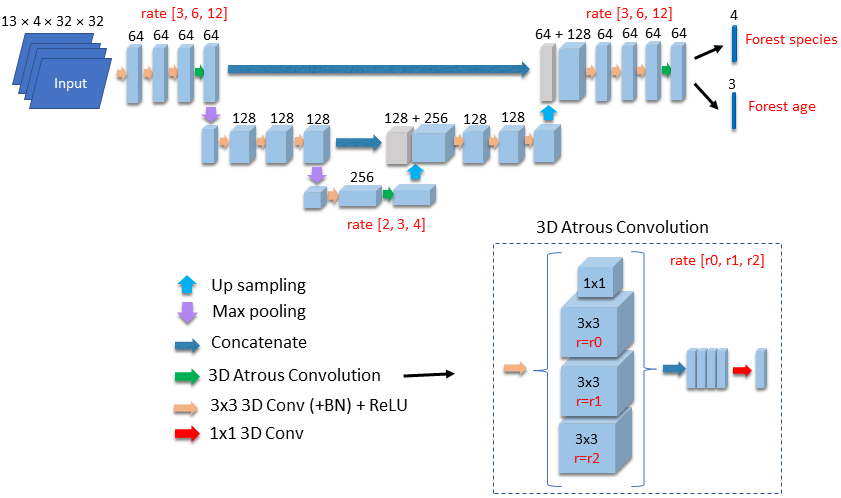
\includegraphics[width=\textwidth]{figs/chap5/model.png}
        \caption{The proposed deep CNN architecture}
        \label{fig:chap5_model}
    \end{subfigure}
    \caption[Workflow and the proposed CNN architecture]{(a) Overall workflow and (b) The proposed deep CNN architecture.}
    \label{fig:chap5_workflow_model}
\end{figure}

\subsubsection*{Forest mapping}
To expedite the forest mapping process, we implemented the Random Forest (RF) model, a widely recognized ensemble machine learning classifier for land-cover and land-use classification \citep{gislason2006random}. The utilization of RF is well-founded not only due to its popularity but also its demonstrated effectiveness in land-cover mapping, particularly when dealing with low-resolution ground-truth data \citep{robinson2021global}. This machine learning approach leverages the strength of ensemble techniques, combining multiple decision trees to enhance accuracy and robustness in the classification of forested areas. The choice of RF aligns with its established success in handling land-cover mapping challenges, making it an efficient solution for our specific context. \par
\subsubsection*{PFTs\slash forest age mapping}

While Random Forest (RF) exhibits commendable performance with low-resolution labeled data, it falls short of achieving superior results compared to our proposed deep learning model, as indicated in Table \ref{tab:chap5_tab2}. The architecture of our proposed network draws inspiration from the UNET architecture \citep{ronneberger2015u} but is intentionally shallower, as depicted in Figure \ref{fig:chap5_model}. To enhance the model's semantic segmentation capabilities, we incorporated 3D Atrous Convolution (3DAConv), a technique proven effective in handling semantic segmentation tasks with coarse annotations \citep{chen2017rethinking}. Atrous convolution, initially introduced in the DeepLab architecture \citep{chen2017deeplab}, involves convolution with upsampled filters. \par

The model comprises an encoder and decoder path backbone. The encoder path encompasses three layers, with the first layer featuring three 3D convolutions (3DConv) followed by a 3DAConv. The second layer contains three 3DConvs, while the last layer consists of one 3DConv followed by a 3DAConv. A 2$\times$2$\times$2 max pooling layer with strides of two follows each encoder layer. Each 3DConv is followed by a rectified linear unit (ReLU), before each ReLU is a batch normalization (BN). Notably, we avoid doubling the number of channels immediately before the max pooling, a departure from the approach introduced in 3D UNET \citep{cciccek20163d}. \par

Moving to the decoder path, ConvTranspose3D is employed for up-convolution to upsample the feature map. A 3DAConv is added at the end of the decoder path. The output dimensions are then reduced to the number of labels through a 1$\times$1$\times$1 3DConv following the last 3DAConv. In our specific case, the number of labels is 4 for Plant Functional Types : Broadleaf, Conifer, Cryptomeria, Chamaecyparis obtusa; and 3 for forest age: young forest ($\le$ 20 years), mature forest (21-50 years), and harvesting age ($\ge$ 50 years). \par

\begin{table}[tbh!]
    \centering
    \caption[Samples, weights for cross-entropy loss training]{Training and validation samples and the corresponding weights for cross-entropy loss function.}
    \begin{tabular}{c c c c}
    \hline
        Class   & Training set  & Validation set & Weight \\ \hline
        \multicolumn{4}{l}{PFTs (number of input images)} \\ \hline
        Broadleaf   & 5017  & 264  & 0.153 \\ 
        Conifer  & 3048  & 160  & 0.252  \\ 
        Chamaecyparis obtusa   & 3191  & 168  & 0.241 \\ 
        Cryptomeria  & 768  & 40  & 1 \\ \hline
        \multicolumn{4}{l}{Forest age (number of input images)} \\ \hline
        Harvesting age   & 4000  & 205  & 0.05 \\ 
        Mature age  & 2095  & 110  & 0.1  \\ 
        Young age   & 186  & 10 & 1 \\ \hline
    \end{tabular}
    \label{tab:chap5_tab1}
\end{table}

The input data is structured with dimensions 13×4×32×32, representing the number of channels, time-series periods, height, and width, respectively. Each input image consists of 32×32 pixels, encompassing a total of 13 channels distributed across three time-series periods. The Digital Elevation Model (DEM) data was incorporated, contributing to the formation of the 4th dimension in the input. Further elaboration on these details is provided in the subsequent section for a more in-depth understanding. \par

Given the imbalanced nature of the training set, as evident in Table \ref{tab:chap5_tab1}, we fine-tuned the model by incorporating a weighted cross-entropy loss function. Specifically, distinct weights were assigned for PFTs and age categories, as outlined in Table \ref{tab:chap5_tab1}.

\subsubsection*{Experiment design and settings}
To assess the performance of the proposed network against Random Forest (RF), 2D UNET, and 3D UNET, we devised an experiment for Plant Functional Types (PFTs) and age mapping using time-series satellite data from Sentinel 1 and 2 in 2018. This data was organized into three distinct periods: January-April (P1), May-August (P2), and October-December (P3). For each period, we conducted a mosaicking and compositing process to create a comprehensive satellite image. Our initial exploration aimed to understand the impact of seasonal changes on PFTs and age mapping performance using RF and 2D UNET. Due to the constraints imposed by the input shape, the assessment of 3D UNET and our proposed model was carried out with data spanning the entire year. To facilitate training with our network and 3D UNET, the input shape needed to be adjusted to 13$\times$4$\times$32$\times$32. This adjustment involved stacking the Digital Elevation Model (DEM) band with the Sentinel 1/2 data in P1, P2, and P3, resulting in input dimensions of each 13$\times$32$\times$32. \par

The performance evaluation of segmentation models was conducted using the Overall Accuracy (OA) score on the validation set. Subsequently, results maps generated by each model underwent visual examination to provide a qualitative assessment.\par

Our deep learning model, implemented in PyTorch, underwent training on an NVIDIA GeForce RTX 3080 Ti GPU. The training process involved 100 epochs, utilizing the Adam optimizer \citep{kingma2014adam} with an initial learning rate of 10\textsuperscript{-5}. The learning rate underwent halving after every 10 epochs.\par

In the context of forest mapping, our approach exclusively employed Sentinel 2 data from June 2018, complemented by 10-meter-resampled DEM data retrieved from GEE. This choice was guided by our observation that June data exhibits minimal slope effects, particularly in regions characterized by higher elevations. The utilization of GEE's API facilitated a seamless implementation, significantly boosting computational efficiency throughout the mapping stages. \par

\section{Experimental results} \label{chap5_result}
For forest mapping, the model accomplished a 94.5\% Overall Accuracy (OA) for the classification of forest and non-forest areas. The resulting forest map, generated by the model, is displayed in Figure \ref{fig:chap5_fig3}. Upon scrutinizing the high-resolution satellite image from Google Earth alongside the overlaid inferred forest map, it becomes evident that the RF model has proficiently and accurately classified the forest pixels using information derived from Sentinel 2 and DEM data. \par

\begin{table}[tbh!]
    \centering
    \caption{The experimental results of UNET and our model.}
    \begin{tabular}{cccc}
    \hline
        \multirow{2}{*}{Model} & \multirow{2}{*}{Time-series period} & \multicolumn{2}{c}{Highest OA (\%)} \\ \cline{3-4}
        ~ & ~ & Species & Age \\ \hline
        \multirow{3}{*}{RF} & P2 & 67.41 & 73.94 \\ 
        ~ & P1 + P2 & 71.68 & 78.66 \\ 
        ~ & P1 + P2 + P3 & 71.65 & 78.68 \\ \hline
        \multirow{3}{*}{2D UNET} & P2 & 59.81 & 65.67 \\ 
        ~ & P1 + P2 & 67.25 & 75.4 \\ 
        ~ & P1 + P2 + P3 & 65.02 & 74.55 \\ \hline
        3D UNET & P1 + P2 + P3 & 76.91 & 80.53 \\ 
        Our model & P1 + P2 + P3 & 77.80 & 81.74 \\ \hline
    \end{tabular}
    \label{tab:chap5_tab2}
\end{table}

\begin{figure}[p]
    \centering
    \begin{subfigure}{\textwidth}
        \centering
        \includegraphics[width=.8\textwidth]{figs/chap5/Forest.png}
        \caption{Forest map in Ena City, Japan}
        \label{fig:chap5_fig3a}
    \end{subfigure}

    \begin{subfigure}{\textwidth}
        \centering
        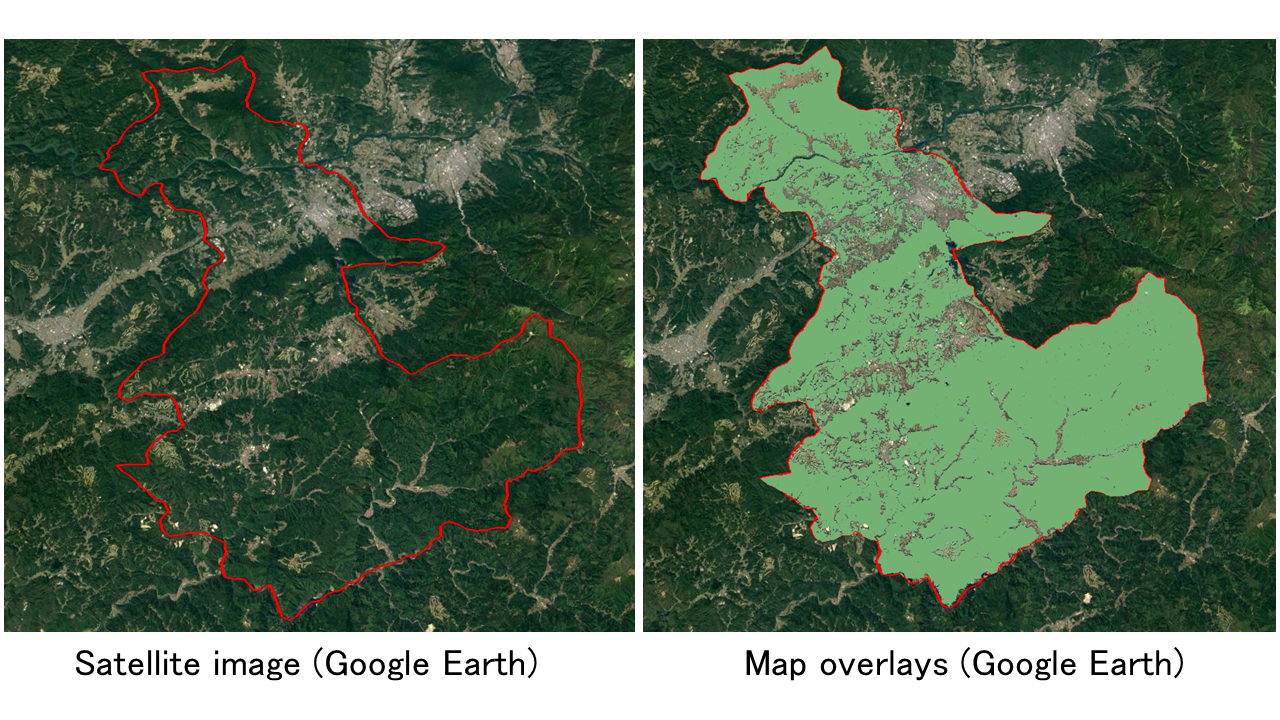
\includegraphics[width=.8\textwidth]{figs/chap5/satimg_overlay.png}
        \caption{Map overlays}
        \label{fig:chap5_fig3b}
    \end{subfigure}
    \caption[Inferred forest map in Ena City]{Inferred forest map in Ena City, Japan \textminus 2018 (OA \textminus 94.5\%)}
    \label{fig:chap5_fig3}
\end{figure}

\begin{figure}[p]
    \centering
    \begin{subfigure}{\textwidth}
        \centering
        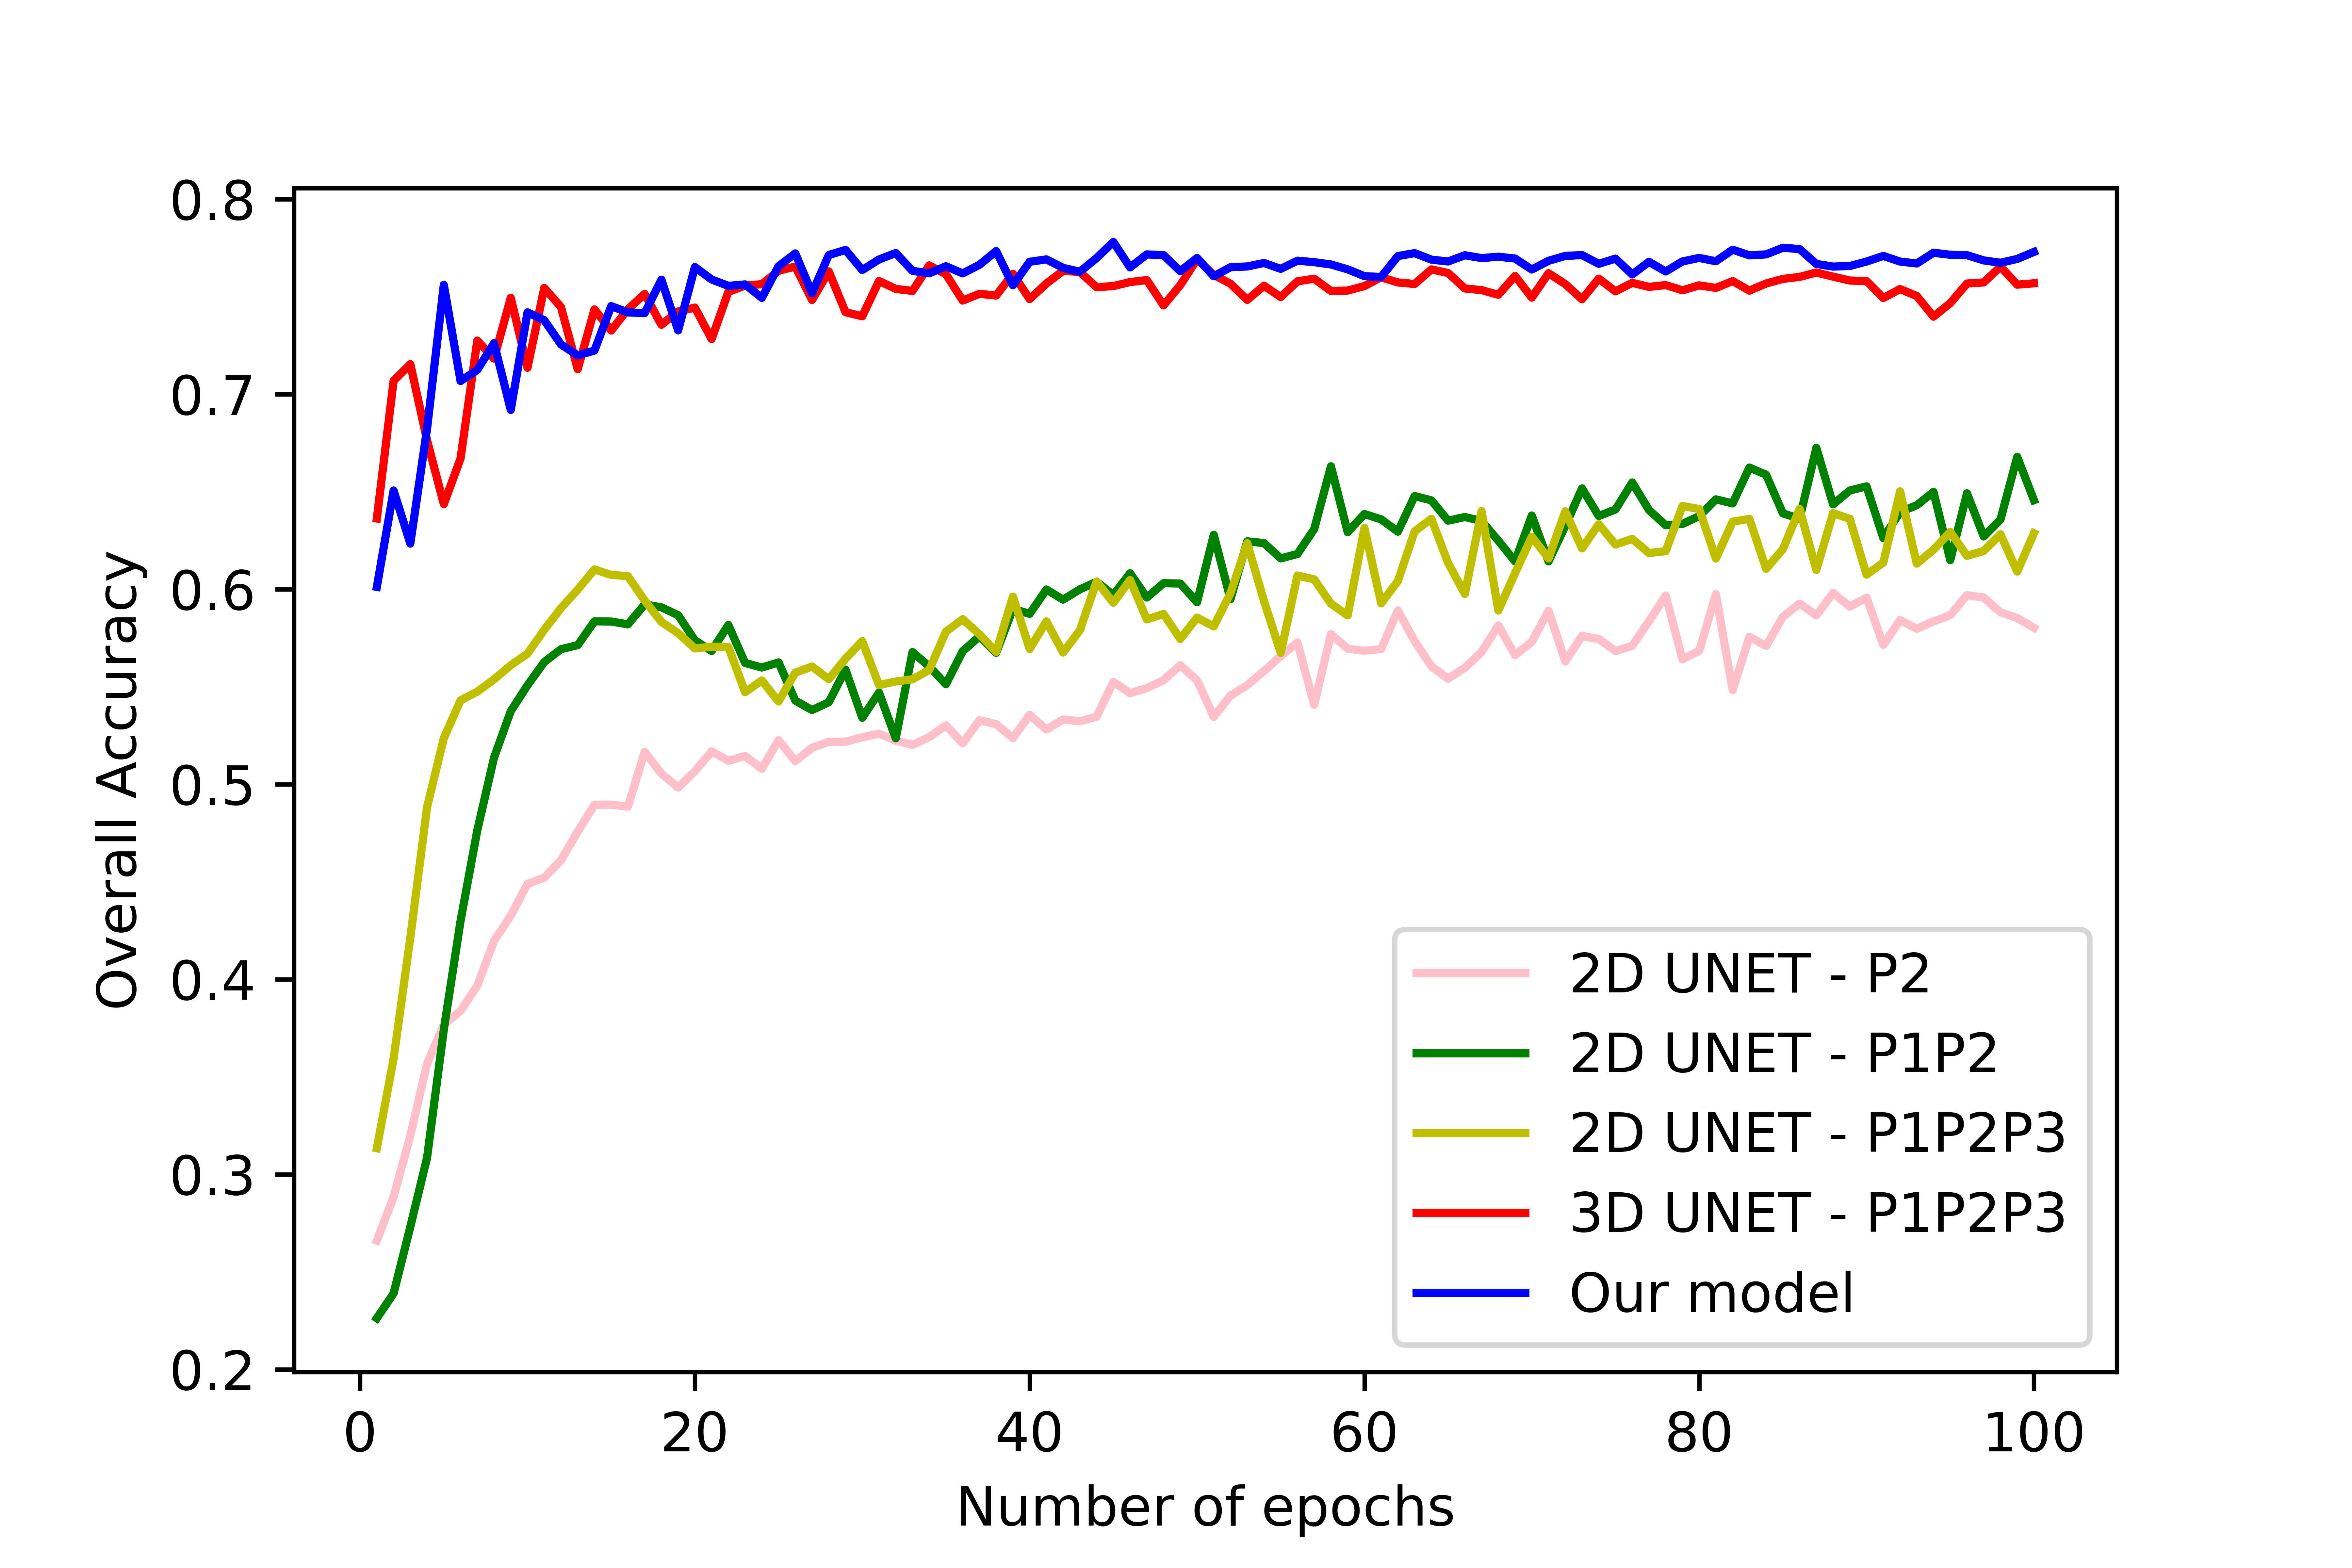
\includegraphics[width=.9\textwidth]{figs/chap5/spec_acc.png}
        \caption{PFTs segmentation.}
        \label{fig:chap5_fig4}
    \end{subfigure}

    \begin{subfigure}{\textwidth}
        \centering
        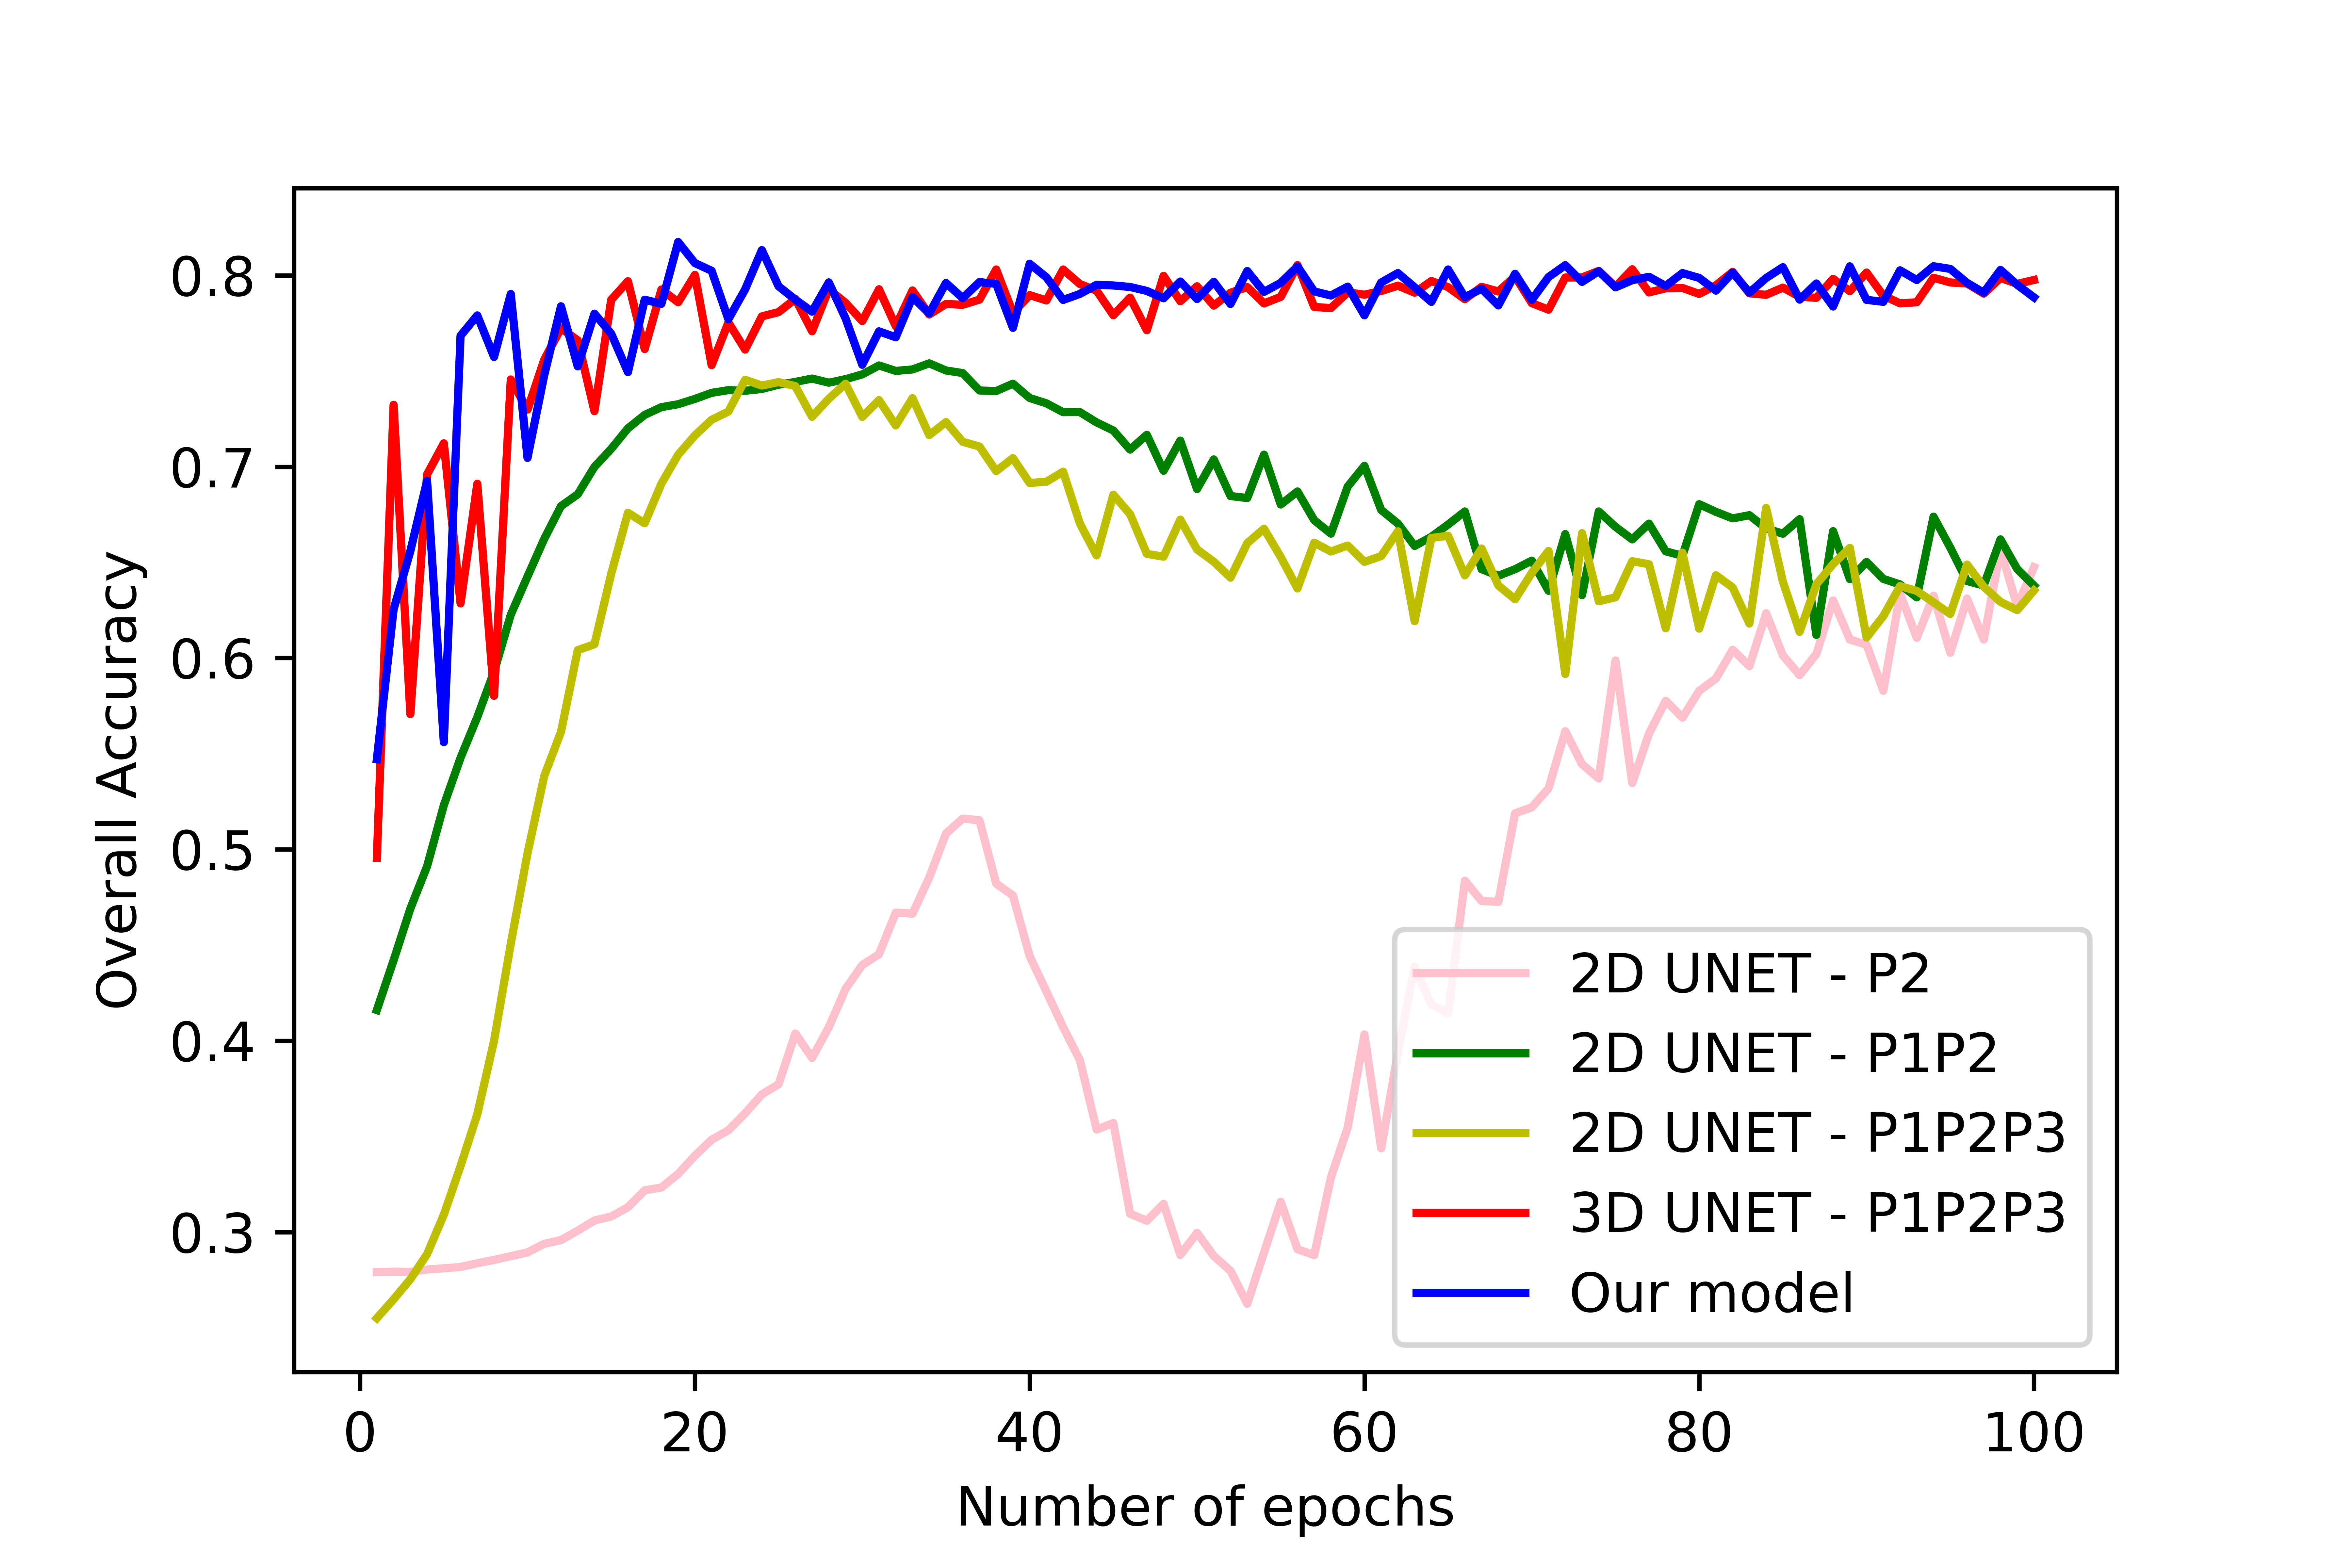
\includegraphics[width=.9\textwidth]{figs/chap5/age_acc.png}
        \caption{Forest age segmentation.}
        \label{fig:chap5_fig5}
    \end{subfigure}
    \caption[Study area and annotated data]{OA profile of PFTs (a) and forest age (b) segmentation}
    \label{fig:chap5_fig45}
\end{figure}


\begin{figure}[tbh!]
    \centering
    \includegraphics[width=.9\textwidth]{figs/chap5/age_map.png}
    \caption[Inferred forest age map in Ena City]{Inferred forest age map in Ena City, Japan \textminus 2018.}
    \label{fig:chap5_fig6}
\end{figure}

\begin{figure}[tbh!]
    \centering
    \includegraphics[width=.9\textwidth]{figs/chap5/spec_map.png}
    \caption[Inferred PFTs map in Ena City]{Inferred PFTs map in Ena City, Japan \textminus 2018.}
    \label{fig:chap5_fig7}
\end{figure}

\begin{figure}[tbh!]
    \centering
    \includegraphics[width=\textwidth]{figs/chap5/other_city.png}
    \caption[PFTs mapping in other regions]{Performance of the proposed method in other regions.}
    \label{fig:chap5_fig8}
\end{figure}

As evident from Table \ref{tab:chap5_tab2}, RF consistently outperformed 2D UNET across all conducted tests. Notably, both the RF and 2D UNET experiments yielded suboptimal results when exclusively relying on data from the P2 period, resulting in the lowest OA for both Plant Functional Types (PFTs) and forest age segmentation. \par

Substantial improvements in OA were observed when extending the time-series scheme from P2 to encompass P1 + P2. However, the addition of P3 to the training set did not yield a significant enhancement in the performance of RF and 2D UNET when compared to the P1 + P2 configuration. This suggests that, for the effective utilization of time-series data in PFTs and forest age segmentation within the study area, the preferable approach involves employing data collected from the January to August period. This is best achieved through an ensemble learning model like RF, or a CNN architecture based on 2D UNET. \par

Despite the minimal impact of P3 data on the performance of RF and 2D UNET, with 3D CNN scheme in 3D UNET and our suggested model, the incorporation of P3 data has significantly elevated the OA in discriminating Plant Functional Types (PFTs) and forest age. The performance comparison of our model, 2D/3D UNET, and RF over 100 epochs is presented in Table \ref{tab:chap3_tab2}, and Figure \ref{fig:chap5_fig45}. Notably, the OA has experienced a substantial improvement, increasing from 71.68\% to 76.91\% with 3D UNET, and reaching 77.80\% with our proposed model for PFTs segmentation. Similarly, for forest age segmentation, the OA has risen from 78.66\% to 80.53\% with 3D UNET, and to 81.74\% with our model. \par

The OA profiles in Table \ref{tab:chap3_tab2}, and Figure \ref{fig:chap5_fig45} underscore the superior performance of our model compared to RF, 2D UNET, and 3D UNET, exhibiting an approximate 6.12\%, 10.55\%, and 0.89\% higher OA for PFTs, and 3.03\%, 6.31\%, and 1.18\% higher OA for forest age segmentation, respectively. \par

Figure \ref{fig:chap5_fig6} depicts the forest age map generated by our model, revealing that the primary harvesting-age areas are predominantly situated in the Northern, Southern, and central parts of the city. Mature-age forests are distributed extensively throughout the region, while smaller areas of young-age forests are scattered across the city from the west to the south. \par

The visual representation of the deduced PFTs map is presented in Figure \ref{fig:chap5_fig7}. Notably, Chamaecyparis obtusa emerges as the prevailing PFTs, exhibiting widespread distribution across the entire region. Cryptomeria, on the other hand, dominates the central Southeast and Northwest sectors of the study area. Broadleaf trees, in majority, are concentrated in the Northeast, Southern, and Northwest segments of the region. The identified Conifer species, while dispersed throughout the Northern and Southern regions, makes a minor contribution from the Northwest portion of the city. \par

Implementing the proposed methodology, we have expanded our mapping efforts to encompass additional cities in Gifu prefecture, namely Nakatsugawa, Mizunami, Toki, and Tajimi, as depicted in Figure \ref{fig:chap5_fig8}. Our approach involved the initial application of the proposed network, followed by the utilization of a straightforward reclassification method. This process enabled the generation of a high-resolution map of Plant Functional Types (PFTs), derived from the pseudo-label output produced by the proposed model.\par

\section{Conclusion} \label{chap5_conclusion}
In this study, by utilizing remote sensing, RF classifier, and deep learning, the approach for forest-related SDG issues monitoring in data-scarce regions has been proposed. We examined the approach in Ena City, Japan and achieved promising results in forest mapping, and PFTs and forest age mapping. Our proposed model outperforms the RF, 2D/3D UNET in PFTs and forest age segmentation with coarse-polygonal ground-truth data. The outcome of this study could be served as an input for further steps to produce high-resolution land cover map for the data-scarce regions. In the future, we will investigate the postprocessing method to improve the map quality from coarse annotations.